\section{Architettura del modulo}

Il modulo cifratore presenta gli ingressi e le uscite visibili in Figura~\ref{fig:layout}.

\begin{figure}[h]
    \centering
    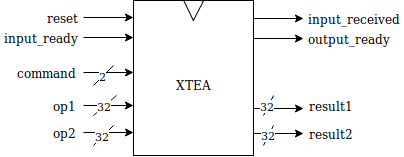
\includegraphics[width=0.4\textwidth]{vhdl_schemi/layout.png}
    \caption{Interfaccia del modulo VHDL}
    \label{fig:layout}
\end{figure}

In input abbiamo:
\begin{itemize}
    \item \code{clock} (1bit): segnale di sincronia;
    \item \code{reset} (1bit): quando alto resetta il modulo alle condizioni iniziali;
    \item \code{input_ready} (1bit): quando alto il modulo può leggere i valori sulle porte \code{command}, \code{op1} e \code{op2};
    \item \code{command} (2bit): operazione da eseguire, deve essere uno tra i valori \code{CONFIGURE_KEYS_0_1}, \code{CONFIGURE_KEYS_2_3}, \code{RUN_ENCRYPT}, \code{RUN_DECRYPT};
    \item \code{op1} (32bit): primo operando;
    \item \code{op2} (32bit): secondo operando.
\end{itemize}
In output abbiamo:
\begin{itemize}
    \item \code{input_received} (1bit): quando alto il modulo segnala di aver letto i valori in input;
    \item \code{output_ready} (1bit): quando alto il modulo segnala completato l'operazione ed è in grado di ricevere nuovi comandi;
    \item \code{result1}, \code{result2} (32bit ciascuno): prima e seconda parte del risultato.
\end{itemize}

Il modulo per poter criptare o decriptare ha bisogno in input di 6 parole a 32bit: quattro appartenenti alla chiave di cifratura, e due appartenenti al messaggio. Abbiamo quindi una prima fase di configurazione, nel quale impostiamo la chiave. Non occorre ripetere questa prima fase se non per cambiare la chiave o dopo un reset. Successivamente possiamo passare il messaggio, due word alla volta, al modulo per effettuare l'operazione richiesta. Questo meccanismo è schematizzato in Figura~\ref{fig:algo}.

\begin{figure}[ht]
    \centering
    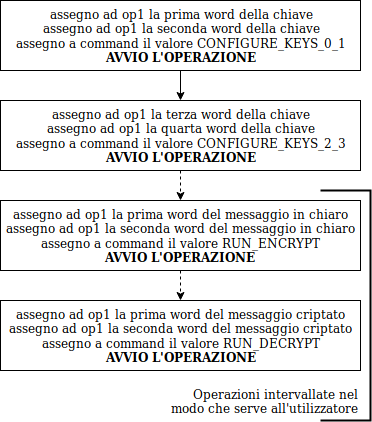
\includegraphics[width=0.36\textwidth]{vhdl_schemi/algo.png}
    \caption{Operazioni del modulo}
    \label{fig:algo}
\end{figure}

Ognuna delle operazioni segue un preciso protocollo illustrato in Figura~\ref{fig:handshake}. Per prima cosa l'utilizzatore scrive sulle porte dei dati e alza \code{input_ready}. Il modulo legge i dati ed abbassa \code{output_ready}. Il ciclo di clock successivo il modulo alza \code{input_received}. A questo punto l'utilizzatore abbassa \code{input_ready}. Una volta che il modulo ha completato l'operazione scrive sulle porte di output i risultati, alza \code{output_ready} ed abbassa \code{input_received}. 

\begin{figure}[ht]
    \centering
    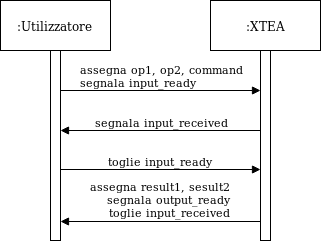
\includegraphics[width=0.36\textwidth]{vhdl_schemi/handshake.png}
    \caption{Protocollo di esecuzione di una qualsiasi operazione}
    \label{fig:handshake}
\end{figure}